\section{Robot Results}

\newcommand{\rrrr}{.3}
\begin{figure*}[b]
\centering
\subfloat[$A=250$, $\sigma=0.15$]{
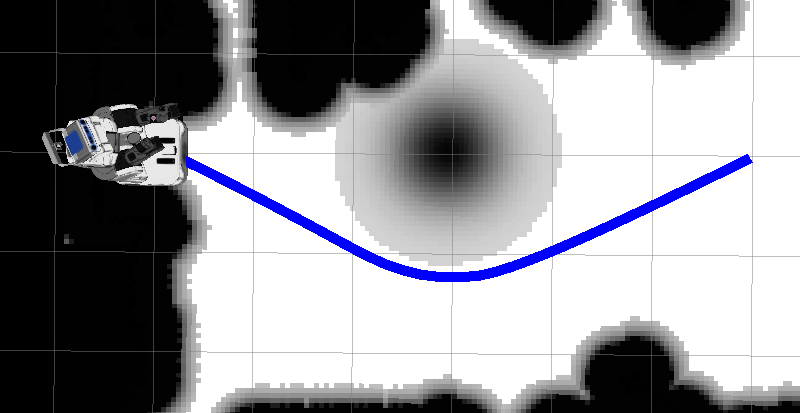
\includegraphics[width=\rrrr\textwidth]{graphix/250-p15.png}
\label{fig:d1}}
\subfloat[$A=250$, $\sigma=0.30$]{
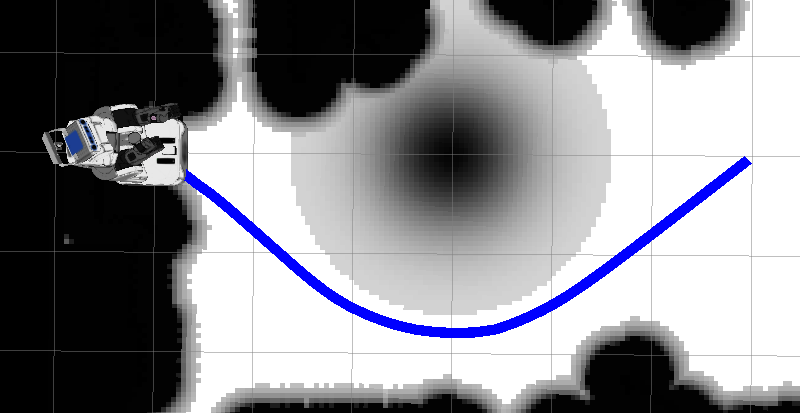
\includegraphics[width=\rrrr\textwidth]{graphix/250-p3.png}
\label{fig:d2}}
\subfloat[$A=250$, $\sigma=0.60$]{
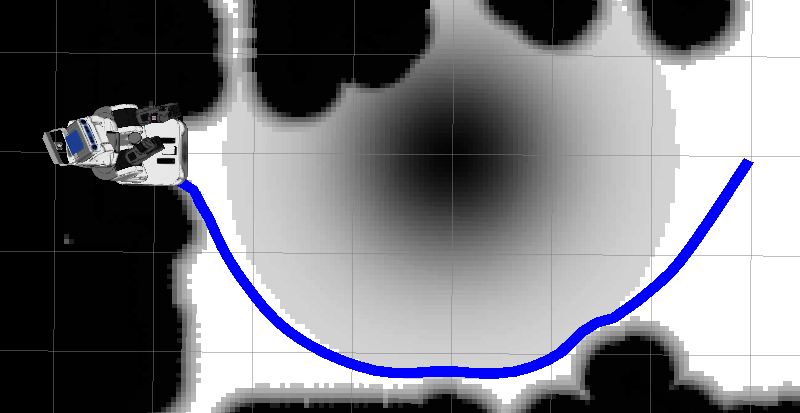
\includegraphics[width=\rrrr\textwidth]{graphix/250-p6.png}
\label{fig:d3}}\\
\subfloat[$A=250$, $\sigma=0.90$]{
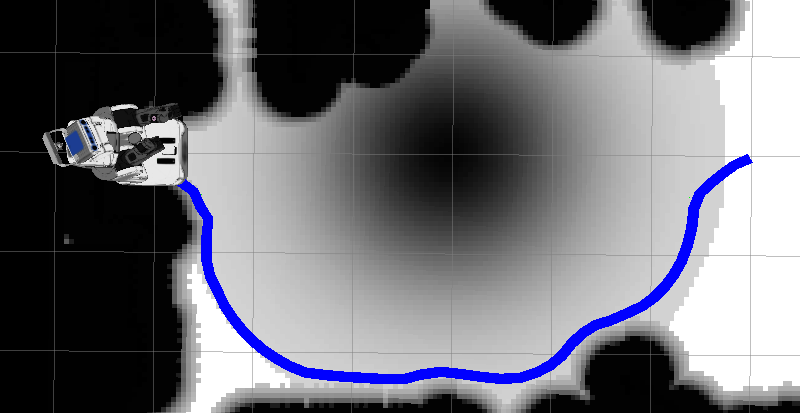
\includegraphics[width=\rrrr\textwidth]{graphix/250-p9.png}
\label{fig:d4}}
\subfloat[$A=250$, $\sigma=1.20$]{
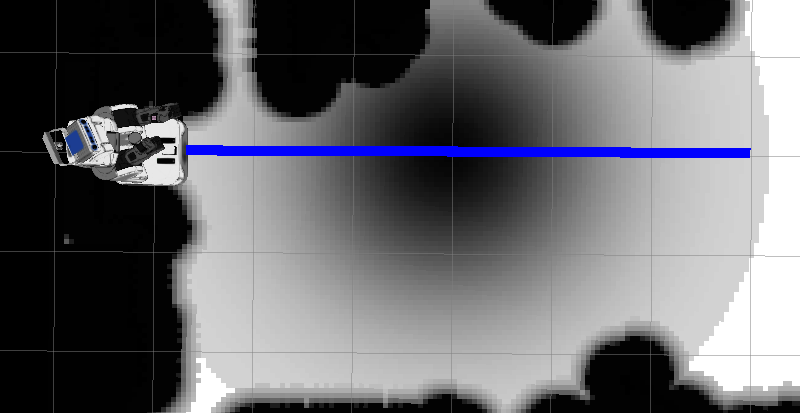
\includegraphics[width=\rrrr\textwidth]{graphix/250-1p2.png}
\label{fig:d5}}
\subfloat[$A=150$, $\sigma=1.20$]{
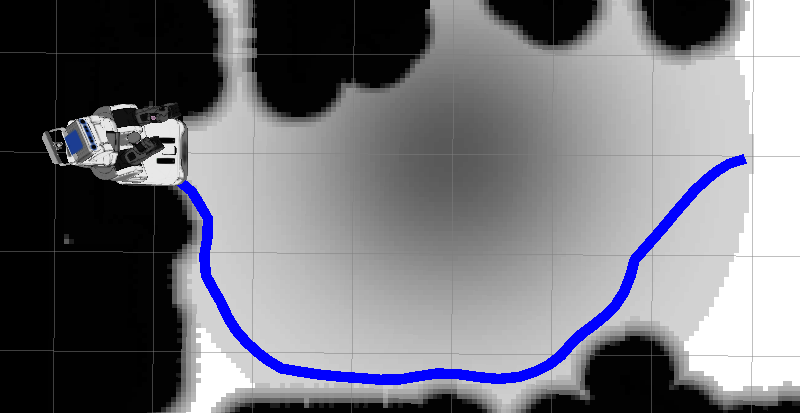
\includegraphics[width=\rrrr\textwidth]{graphix/150-1p2.png}
\label{fig:d6}}
\caption{Real plans generated by the ROS Navigation Stack - As the variance increases (a)-(d), the path gets further from the obstacle. However, in (e) when the variance is over 1, the path reverts to straight through. }
\label{fig:realdata}
\end{figure*}
